\documentclass{article}
\usepackage[letterpaper, margin=1in]{geometry}
\usepackage{parskip} % Add space between paragraphs
\setlength{\parskip}{0.9em}

\usepackage{fancyvrb}
\usepackage{amsmath}
\usepackage{graphicx}
\usepackage[most]{tcolorbox}
\tcbset{colback=white, sharp corners, colframe=gray, boxsep=2pt, boxrule=0.2pt, before
skip=10pt, after skip=5pt}

\usepackage{titling}
\title{Project 1: Density Estimation and Classification}
\author{Youmi Koh}
\date{Aug 30, 2023}

\makeatletter
\def\@maketitle{
\newpage
 \null
 \vskip 0em
 \begin{center}
  {\LARGE \@title \par}%
  {\large \@author \par}%
  {\large \@date \par}%
 \end{center}%
 \vskip 1.8em}
\makeatother

\usepackage{fancyhdr}
\fancypagestyle{plain}{%  the preset of fancyhdr
    \fancyhf{} % clear all header and footer fields
    % \fancyfoot[L]{\thedate}
    \fancyhead[L]{CSE575 - Fall 2023}
    \fancyhead[R]{Student ID: 1231025486}
}

\begin{document}
\maketitle
\noindent
This project involves implementing supervised, unsupervised, and deep learning techniques for density estimation and classification.  The project focuses on a subset of the MNIST dataset
containing images of digits "0" and "1", and demonstrates feature extraction, parameter calculation, implementation of Naïve Bayes classifiers, and prediction of labels for the test data using
the classifiers. Finally, accuracy of the predictions are calculated and observations are presented.

\subsection*{Maximum Likelihood Estimation}

The average brightness (\texttt{f1}) and standard deviation of brightness (\texttt{f2}) of images are extracted as features from the training data. We assume that these two features are independent and that each image is drawn from a normal distribution. Images depict either the digit zero (\texttt{d0}) or one (\texttt{d1}), and these digit labels are used to estimate the parameters of a normal distribution ($\texttt{mean},\texttt{var}$) for each feature/digit pair.

Likelihood function for a normal distribution: ${\displaystyle L(\mu, \sigma) = p(X\mid\mu,\sigma) = \left(\frac{1}{\sigma\sqrt{2\pi}}\right)^n \prod_i^n \exp\left(-\frac{(x_i - \mu)^2}{2\sigma^2} \right)}$

Log-likelihood function for convenience: ${\displaystyle l(\mu, \sigma) = \operatorname{log}p(X\mid\mu,\sigma) = -n \operatorname{log}(\sigma\sqrt{2 \pi}) \sum_i^n \exp\left(-\frac{(x_i - \mu)^2}{2\sigma^2} \right)}$

Maximum likelihood estimates for mean $\mu$ and variance $\sigma^2$:$$
\begin{array}{lcr}
{\displaystyle \hat{\mu} = {\underset {\mu}{\operatorname {argmax} }}\ l(\mu, \sigma) = \frac{1}{n} \sum_i^n {x_i}}
&& {\displaystyle \hat{\sigma} = {\underset {\sigma}{\operatorname {argmax} }}\ l(\mu, \sigma)\ \Rightarrow\ \widehat{\sigma^2} = \frac{1}{n} \sum_i^n {(x_i-\mu)^2}}
\end{array}
$$

In the results below, the mean of \texttt{f1} (average brightness) is notably higher for \texttt{d0} than \texttt{d1}, which suggests the images of zeroes are generally brighter than images of ones. The mean of \texttt{f2} (standard deviation of brightness) is also significantly higher for \texttt{d0} than \texttt{d1}, indicating that the brightness values within each image of zeroes vary more widely. Variance for \texttt{d0} is larger than \texttt{d1} for both features, and this may impact the derived classifier.

\begin{center}
\begin{tcolorbox}[width=0.9\textwidth]
\begin{verbatim}
    Mean_of_feature1_for_digit0: 44.20389362244898
    Variance_of_feature1_for_digit0: 116.7009513315956
    Mean_of_feature2_for_digit0: 87.41907699909902
    Variance_of_feature2_for_digit0: 102.46490855207279

    Mean_of_feature1_for_digit1: 19.43962244897959
    Variance_of_feature1_for_digit1: 31.98890083543315
    Mean_of_feature2_for_digit1: 61.44770668123185
    Variance_of_feature2_for_digit1: 83.54555141482662
\end{verbatim}
\end{tcolorbox}
\end{center}
\;
\subsection*{Naive Bayes Classification}

The above estimates serve parameters in the normal probability density functions that calculate conditional probabilities for naive Bayes classification.
$${\displaystyle p(\texttt{digit}\mid \texttt{features} )={\frac {p(\texttt{digit})\cdot p(\texttt{features}\mid\texttt{digit})}{p(\texttt{features})}}\, \Leftrightarrow \, \text{posterior}={\frac {{\text{prior}}\times {\text{likelihood}}}{\text{evidence}}} }$$

Although \texttt{f1} and \texttt{f2} are not necessarily independent, we assume that these features are conditionally independent given a class \texttt{d}. This assumption allows us to simplify the likelihood function to the product of the likelihoods of each feature given the digit.
$$
\begin{array}{cccl}
p(\texttt{f}_i\mid \texttt{f}_j, \texttt{d}_k)=p(\texttt{f}_i\mid \texttt{d}_k) \Rightarrow & p(\texttt{d}_k\mid \texttt{f1},\texttt{f2}) &\propto& p(\texttt{d}_k,\texttt{f1}, \texttt{f2})\\
&&\propto& p(\texttt{d}_k)\cdot p(\texttt{f1}\mid \texttt{d}_k) \cdot p(\texttt{f2}\mid \texttt{d}_k)
\end{array}\;\ k \in\{0,1\}
$$
Prior probabilites $p(\texttt{d}_k)$ are derived from the training data, and the likelihood conditional probabilities $p(\texttt{f}_i\mid \texttt{d}_k)$ are calculated using the estimated normal distribution parameters $\texttt{mean}_{(\texttt{f;d})}$ and $\texttt{var}_{(\texttt{f;d})}$. Then posterior probabilities are calculated for each digit, and the digit with the highest probability is selected as the classification.

\subsection*{Accuracy}
Despite the naive assumption, the classifier performs well on the test data.

\begin{center}
\begin{tcolorbox}[width=0.9\textwidth]
\begin{verbatim}
    Accuracy_for_digit0testset: 0.9173469387755102
    Accuracy_for_digit1testset: 0.9233480176211454
\end{verbatim}
\end{tcolorbox}
\end{center}

\texttt{d1} slightly outperforms \texttt{d0} as a result of the smaller MLE variances. The below plot illustrates density contours for digits (0,1) learned from the training set, and highlights the overlay of test data. We can see \texttt{d1} density is more concentrated, and the spread of test set data that was misclassified.

\begin{figure}[h]
\centering
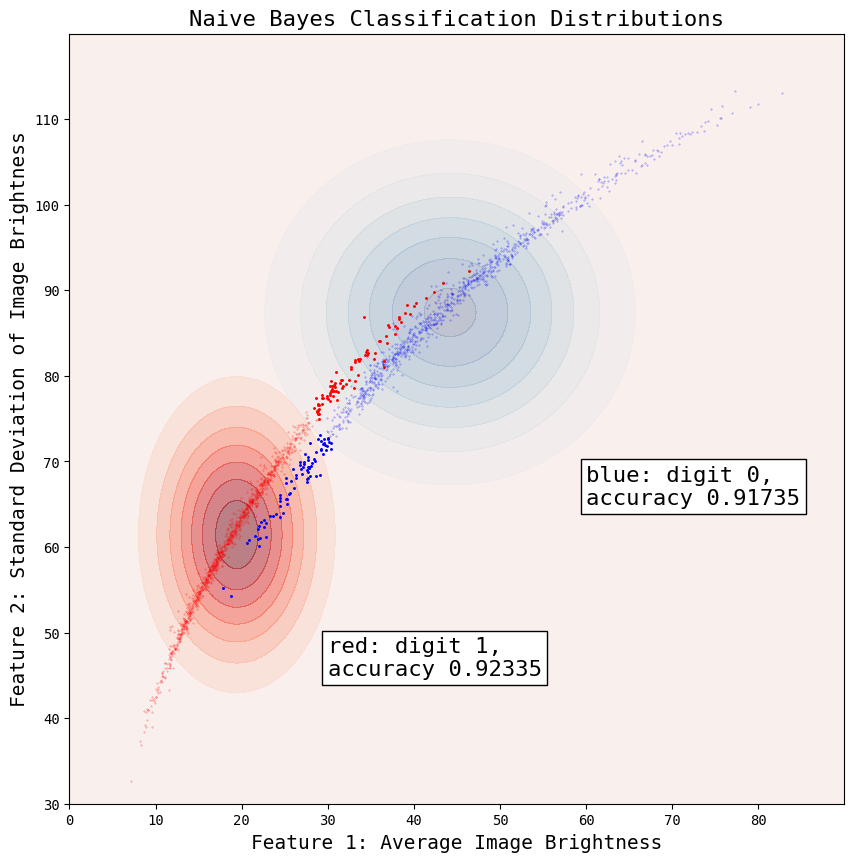
\includegraphics[width=0.75\textwidth]{output.png}
\end{figure}

\end{document}
